\documentclass{article}
\usepackage{listings}
\usepackage{color} %red, green, blue, yellow, cyan, magenta, black, white
\definecolor{mygreen}{RGB}{28,172,0} % color values Red, Green, Blue
\definecolor{mylilas}{RGB}{170,55,241}

\usepackage{booktabs}
\usepackage{pgfplots}
\usepackage{pgfplotstable}
\usepackage{movie15}
\usepackage{graphicx}
\usepackage{amsmath}
\usepackage{float}
\usepackage{physics}
\usepackage[colorlinks=true, linkcolor=blue]{hyperref}
\usepackage[english]{babel}
\selectlanguage{english}
\usepackage[utf8]{inputenc}
\usepackage[svgnames]{xcolor}
\usepackage{subfig}
\usepackage{listings}
\usepackage{afterpage}
\pagestyle{plain}
\usepackage{graphicx}
\usepackage[export]{adjustbox}

\definecolor{dkgreen}{rgb}{0,0.6,0}
\definecolor{gray}{rgb}{0.5,0.5,0.5}
\definecolor{mauve}{rgb}{0.58,0,0.82}
\definecolor{carrotorange}{rgb}{0.93, 0.57, 0.13}

\lstset{language=C,
    frame=tb,
    backgroundcolor=\color{white},   
    commentstyle=\color{dkgreen},
    keywordstyle=\color{blue},
    numbers=none,
    stringstyle=\color{carrotorange},
    basicstyle=\footnotesize,
    breakatwhitespace=false,         
    breaklines=true,                 
    captionpos=b,                    
    keepspaces=true,                 
    numbersep=5pt,                  
    showspaces=false,                
    showstringspaces=false,
    showtabs=false,                  
    tabsize=2,
    language=C
}

\usepackage{here}

\textheight=21cm
\textwidth=17cm
%\topmargin=-1cm
\oddsidemargin=0cm
\parindent=0mm
\pagestyle{plain}

\usepackage{color}
\usepackage{ragged2e}

\global\let\date\relax
\newcounter{unomenos}
\setcounter{unomenos}{\number\year}
\addtocounter{unomenos}{-1}
\stepcounter{unomenos}
\gdef\@date{ Course \arabic{unomenos}}

\begin{document}
\begin{titlepage}
\begin{center}
\vspace*{-1in}
\begin{figure}[htb]
\begin{center}

\includegraphics[width=8cm]{UU_logo.jpg}
\end{center}
\end{figure}

DEPARTMENT OF INFORMATION TECHNOLOGY - \@date\\
\vspace*{0.15in}
HIGH PERFORMANCE PROGRAMMING - ASSIGNMENT 4:\\The Barnes-Hut Method \\
\vspace*{0.3in}
\begin{large}
KIERAN BARBER\\
\end{large}
\vspace*{0.1in}
\begin{Large}
PANAGIOTIS PAPIAS\\
\end{Large}
\vspace*{0.1in}
\rule{80mm}{0.1mm}\\
\vspace*{0.1in}
\begin{large}
Teacher \\
Sverker Holmgren
\end{large}
\end{center}
\end{titlepage}

\newcommand{\CC}{C\nolinebreak\hspace{-.05em}\raisebox{.4ex}{\tiny\bf +}\nolinebreak\hspace{-.10em}\raisebox{.4ex}{\tiny\bf +}}
\def\CC{{C\nolinebreak[4]\hspace{-.05em}\raisebox{.4ex}{\tiny\bf ++}}}

\tableofcontents
\newpage
\section{The Problem}
For this assignment, we are going to implement a program that will calculate the evolution of N particles in a gravitational simulation, whereby we are given an initial set of particles. The simulation will be done in 2 spatial dimensions with an $x$ and $y$ coordinate. 
\\\\
To help describe the evolution of these particles, we use Newton's law of gravitation in two dimensions, which states that the force exerted on particle $i$ by particle $j$ is given by
\\\\
    $$\boldsymbol{f}_{ij} = -\frac{Gm_{i}m_{j}}{\|\boldsymbol{r}_{ij}\|^{3}}\boldsymbol{r}_{ij}.$$
\\\\
where G is the gravitational constant, $m_{i}$ and $m_{j}$ are the masses of the particles, and $\boldsymbol{r}_{ij}$ is the distance vector given by $\boldsymbol{x}_{i} -\boldsymbol{x}_{j}$ with $\boldsymbol{x}_{i}$ being the position of particle $i$. 
\\\\
We will make use of the following force equation (Plummer Sphere Force Equation) to describe the forces on the particles. The force on particle $i$ is given by
\\\\
    $$\boldsymbol{F}_{i} = -Gm_{i}\sum_{j = 0, j \neq i}^{N-1}\frac{m_{j}}{(\|\boldsymbol{r}_{ij}\| + \epsilon_{0})^{3}}\boldsymbol{r}_{ij}.$$
\\\\
where $\epsilon_{0}$ is a smoothing parameter and in the computations, we used the value $\epsilon = 10^{-3}$.
\\\\
To update the particle positions, we use the Euler Symplectic Time Integration method. The equations describing this are
\\\\
\begin{cases}
    $\boldsymbol{a}_{i}^{n} = \frac{\boldsymbol{F}_{i}^{n}}{m_{i}}$;
    \\
    $\boldsymbol{u}_{i}^{n+1} = \boldsymbol{u}_{i}^{n} + \Delta t\boldsymbol{a}_{i}^{n}$;
    \\
    $\boldsymbol{x}_{i}^{n+1} = \boldsymbol{x}_{i}^{n} + \Delta t\boldsymbol{u}_{i}^{n+1}$,
\end{cases}
\\\\
where $\Delta t$ is the time step size, $\boldsymbol{a}_{i}$ is the acceleration of particle $i$, $\boldsymbol{u}_{i}$ is the velocity and $\boldsymbol{x}_{i}$ is the position of particle $i$. In the computations, we used $\Delta t = 10^{-5}$. The value of G depends on N and is given by $G = 100/N$.
\newpage
\section{The Solution}
\begin{figure}[htb]
\begin{center}
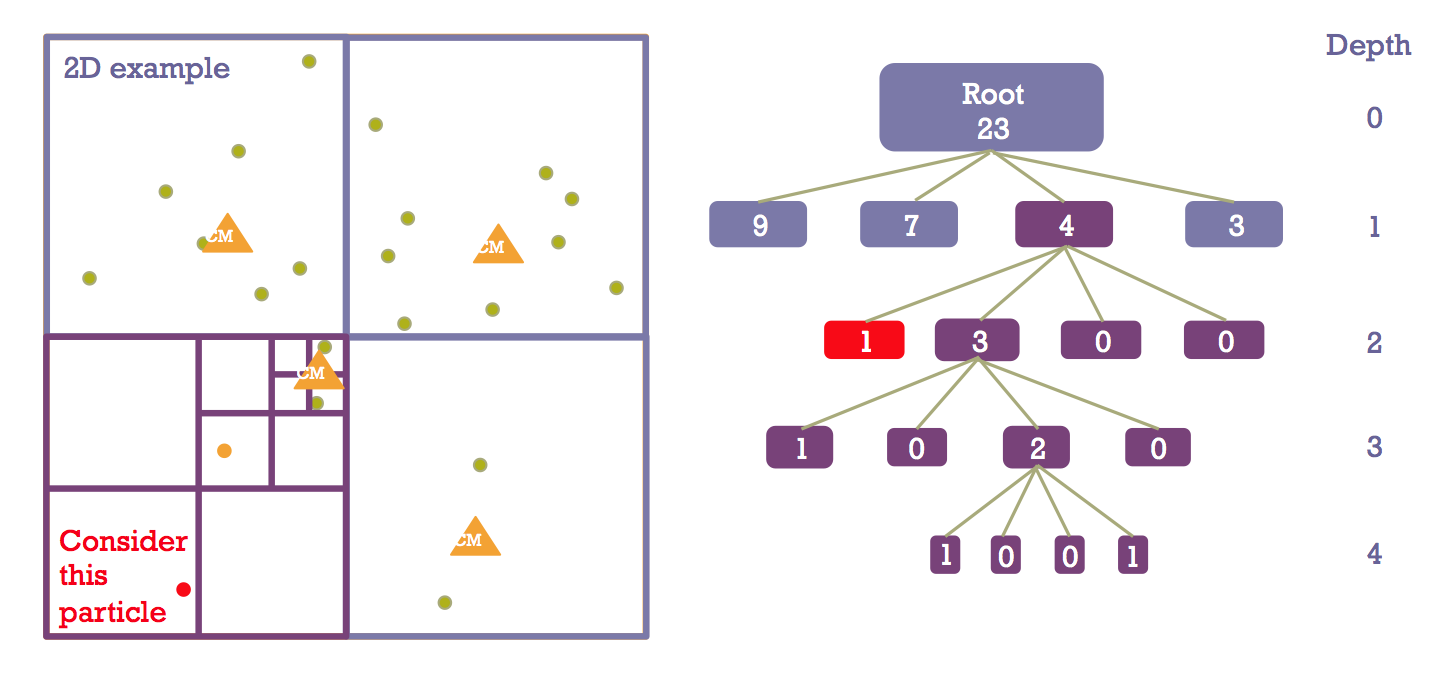
\includegraphics[width=8cm]{tree_walk.png}
\caption{Diagram of Barnes Hut method}
\end{center}
\end{figure}
To solve the N body problem, we implemented something known as the Barnes-Hut algorithm. The purpose of this algorithm is to improve computation time, whilst maintaining a high level of accuracy. The idea is to take a group of particles located near to each other and instead of computing forces individually, we do it as group and calculate the force they exert on another particle. To maintain accuracy, we only do this for groups that are far away from the particle. This means that if we have M particles in the group, then we save M-1 force calculations in which we need to compute. 
\\\\
For this assignment, we initially  chose to separate the code into files that represented each section of code we required. We chose to do this for a cleanliness aspect. These files are: 
\begin{itemize}
    \item \verb|box_bounds.c| \verb|box_bounds.h|
    \item forces.c forces.h
    \item galsim.c
    \item particle.c particle.h
    \item quad.c quad.h
    \item vector.c vector.h
    \item Makefile
    \item timings.sh
\end{itemize}
\subsection{Quadtree}
To begin with, we constructed the quadtree in the file quad.c. We take an empty tree and insert the particles iteratively, one by one. The first case involves simply adding a particle to an empty tree. The other cases involve recursion. 
\\\\
So in case one, if the tree is empty, we insert the particle into the root node. When we add the particle here, we must also set its mass and centre of mass at the same time, which in this case is easy since it will take the same value as the single particle. 
\begin{figure}[htb]
\begin{center}
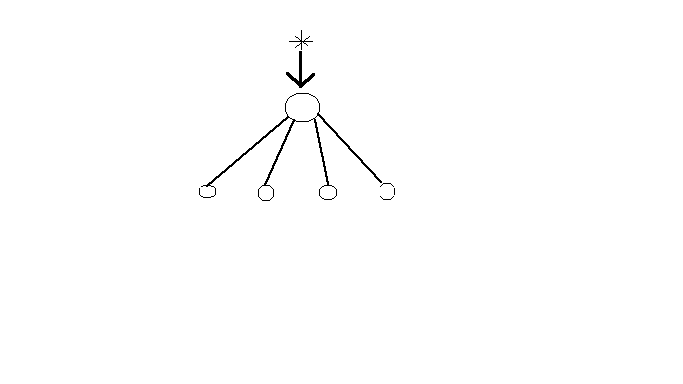
\includegraphics[width=8cm]{empty_tree.png}
\caption{Diagram of Empty Tree}
\end{center}
\end{figure}
\\\\
The second case, is that we traverse the tree and we end up on a node that is taken, but with no children. In this scenario, we must take the particle to one of the children and then also take the particle that was in the node into one of the other children. If they end up going to the same place again, then we traverse the tree until they are split into separate nodes. We update the mass and centre of mass for each particle at the same time. 
\begin{figure}[htb]
\begin{center}
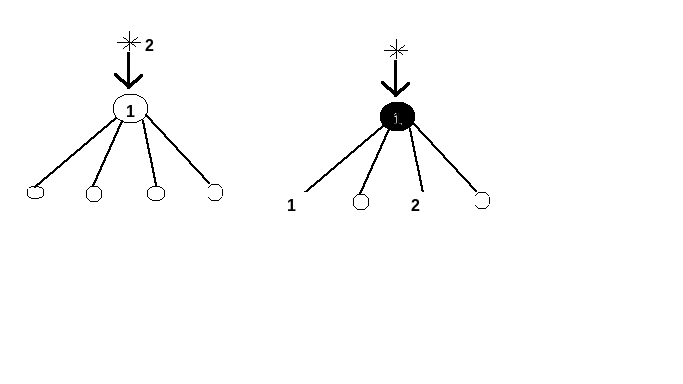
\includegraphics[width=8cm]{node_no_children.png}
\caption{Diagram of Node with no children}
\end{center}
\end{figure}
The final case in our code is if we already have a particle in one of the children spots but not all of them. In this scenario, we simply need to traverse the tree until we get to the node with space in its children so that this new particle can be placed here. 
\\\\
The code for this section has been placed in the appendix (A1).
\begin{figure}[htb]
\begin{center}
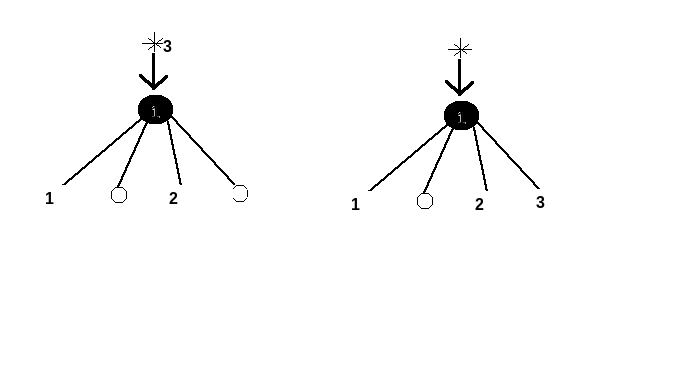
\includegraphics[width=8cm]{children.png}
\caption{Diagram of Node with children}
\end{center}
\end{figure}
\\\\
\newpage
\subsection{Forces}
In order to compute the forces we need the quadtree, which is built in quad.c, the particle that the force is computing for, and \verb|theta_max|. Again, we have three scenarios in which we need to compute the forces. The first case is that if the tree is NULL then we have no forces in which there is any interaction. 
\\\\
The next case we have is if the particle that is inserted next in the tree is firstly not in a particular boxed region and either far enough away from this boxed region or it has no children, then we can compute the force applied to it from the boxed region. We have to check this, since care is needed to not include the particle itself. \\\\
The final case we have is to compute the forces of each child and then sum these together to compute the force of the node. 
\\\\
The code for the forces is in the appendix, under section (A2).

\subsection{Other Files}
The purpose of \verb|box_bounds.c| is to house a function called \verb|vector_in_box| which is called into functions in forces. This function is used to determine whether a particle traversing the quad tree is within the bounds of a certain node. 
\\\\
Since our code has been separated out into different files, galsim.c only holds particle position updates and updates outside of the main function. In the main function, we take the arguments from the user, and call the compute force functions to get our output. 
\\\\
The particle.c file contains functions that help read and write the particle data involved.
\\\\
The vector.c file contains the \verb|r_vector| and norm functions that helps compute the forces on the particles. 
\\\\
For convenience, we have included a timings.sh file that runs the different versions of Makefile on different optimisation flags.
\newpage
\section{CPU Configuration}
\begin{verbatim}
Architecture:        x86_64
CPU op-mode(s):      32-bit, 64-bit
Byte Order:          Little Endian
CPU(s):              8
On-line CPU(s) list: 0-7
Thread(s) per core:  2
Core(s) per socket:  4
Socket(s):           1
NUMA node(s):        1
Vendor ID:           GenuineIntel
CPU family:          6
Model:               142
Model name:          Intel(R) Core(TM) i5-8250U CPU @ 1.60GHz
Stepping:            10
CPU MHz:             700.041
CPU max MHz:         3400,0000
CPU min MHz:         400,0000
BogoMIPS:            3600.00
Virtualization:      VT-x
L1d cache:           32K
L1i cache:           32K
L2 cache:            256K
L3 cache:            6144K
NUMA node0 CPU(s):   0-7

(Ubuntu 7.4.0-1ubuntu1~18.04.1) 7.4.0

\end{verbatim}
\newpage
\section{Performance and Discussion}
\subsection{Timings - Getting up to speed}
\begin{center}
\begin{tabular}{|c|c|c|c|c|}
\hline
Version & -OO & -O3 & -Ofast -march=native & -O4\\
\hline
V1.1 & 24.304349 & 13.470492 & 12.901046 & 13.474097\\
V1.2 & 24.204505 & 2.549037 & 2.035497 & 2.542937\\
V1.3 & 12.155917 & 2.900762 & 2.836586 & 2.902077\\
\hline
\end{tabular}
\end{center}
Since the functions are now spread over several files, we need to check that we have as efficient timings as in the version without the Barnes Hut algorithm. To test this, we first use a check file to make sure our results are accurate. The timing results of this we omit.
\\\\
The next step is to then compare timing results to that of previous results we have obtained. 
\\\\
Version 1.1 above is based on previous results from which we can compare. This involves using 3000 particles and 100 time steps. For this version (1.1) we have the functions \verb|r_vector|, norm and norm3 in the file vector.c, with the force functions from a previous version now in the forces.c file and all are called to the galsim.c main file. This shows some significant loss in computation time compared to a previous version. We now take all the vector functions into the forces.c file to see if this helps with computation time.
\\\\
The next version (1.2) does indeed appear to speed up the computation times significantly for the flags apart from -O0. 
\\\\
Finally, in version (1.3), we make a comparison with the quadtree implemented for 3000 particles and 100 time steps to see how this compared. Before testing this, we ran this with $\theta$ set to zero first to ensure we maintained accuracy before optimising for $\theta$. This is allowed an accuracy of up to $10^{-3}$. The optimal value we obtained for $\theta$ is 0.25. This ran only marginally slower for all the flags apart from -O0, where this ran twice as fast. 
\subsection{Timings - Which section to focus on}
Before we begin optimisation of the code, we look to which part of the code requires the most optimisation. We split the code into computing quadtree build time and forces computation time. We focused on the -Ofast and -march=native optimisation flags. The quadtree took 0.144213 seconds to compute for 5000 particles with 100 time steps. The forces took 5.302154 seconds to compute with the same parameters. On this evidence, we will look to focus our optimisations on computing the forces, since this took approximately $97\%$ of the computation time.
\subsection{Timings - Optimised}
\begin{center}
\begin{tabular}{|c|c|c|c|c|}
\hline
Version & -OO & -O3 & -Ofast -march=native & -O4\\
\hline
V2.1 & 23.720430 & 5.669060 & 5.449106 & 5.842755\\
\hline
V2.2 & 23.545072 & 5.277797 & 4.420938 & 5.303275\\
\hline
V2.3 & 18.177161 & 5.102843 & 4.393660 & 5.105376\\
\hline
V2.4 & 17.941679 & 4.841763 & 4.289874 & 4.820603\\
\hline
\end{tabular}
\end{center}
Version 2.1 here involves having all the function calls in forces aside from \verb|vector_in_box|, which has been left out in the \verb|box_bounds.c| file. 
\\\\
This is where our first optimisation is. In Version 2.2, we chose to move \verb|vector_in_box| in to the forces file. This does indeed speed up the computation times for all apart from the -O0 flag.
\\\\
In Version 2.3, we made an optimisation involving making a modification to \verb|theta_bounds|, which in turn meant we would have to make a modification to \verb|quad_force|. We took in two extra arguments in \verb|theta_bounds|, where we take pointers so that we only have to compute norm(r) just the once. This has some computational time effects for each flag, but mostly -O0. 
\begin{center}
    Version 3 - \verb|theta_bounds|
\end{center}
\begin{lstlisting}{language=C}
    int theta_bounds(quadtree_t* tree, particle_t particle, double theta_max, vector_t* r, double* n) {
    double xwidth = tree->box.xupper - tree->box.xlower;
    *r = r_vector(tree->centre_of_mass, particle.position);
    *n = norm(*r);

    if(xwidth / *n < theta_max) {
        return 1;
    }
    else {
        return 0;
    }
}
\end{lstlisting}
\\\\
In version 2.4, the final optimisation involved using our final \verb|theta_bounds| function, where we switched from dividing to multiplying. We did this since dividing is computationally more expensive than multiplying. This made for a minimal increase in performance on all the flags.
\begin{center}
    Version 4 - \verb|theta_bounds|
\end{center}
\begin{lstlisting}{language=C}
    int theta_bounds(quadtree_t* tree, particle_t particle, double theta_max, vector_t* r, double* n) {
    *r = r_vector(tree->centre_of_mass, particle.position);
    *n = norm(*r);

    return tree->box.xupper - tree->box.xlower < theta_max * (*n);
}
\end{lstlisting}
\begin{figure}[htb]
\begin{center}
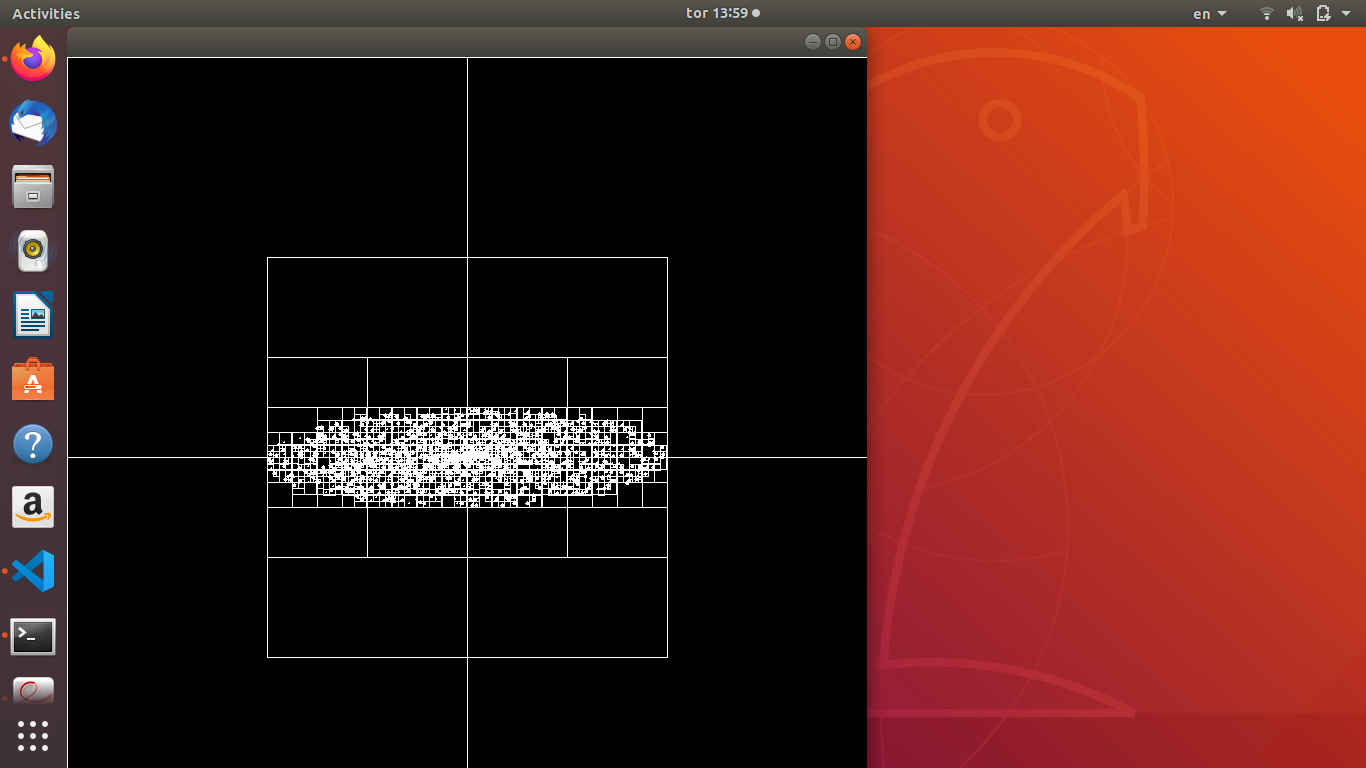
\includegraphics[width = 10cm, trim=2.2cm 0 {17.5cm\width} 4cm, clip]{squarespace.jpg}
\caption{A simulation of a galaxy}
\end{center}
\end{figure}
\newpage
\subsection{Unsuccessful Optimisations}
We tried a few more optimisations on top of the ones described above, however, these were unsuccessful.
\\\\
The first of these optimisations was to bring the forces.c file into the galsim.c file to see if there could be further time reductions in computation time. When this didn't produce any better time performance we decided to also bring in the quad.c file into the galsim.c file so that they are all located in the same place. Both were unsuccessful optimisations.
\newpage
\subsection{Complexity}
Finally, below we have a plot outlining the computation times measured against $O(Nlog(N))$.
\begin{figure}[htb]
\begin{center}
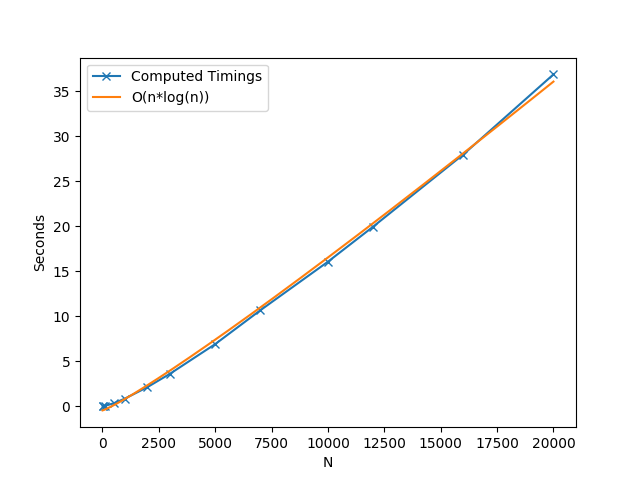
\includegraphics[width=8cm]{nlogn.jpg}
\caption{Time Complexity Plot}
\end{center}
\end{figure}
\\\\
We have then compared this method to the naive approach to see how much more effective it is as we increase the number of particles. As we can see, to begin with the naive approach has better computation time, but as the number of particles increases, the Barnes Hut algorithm shows its potential to calculate these things much more efficiently. 
\begin{figure}[htb]
\begin{center}
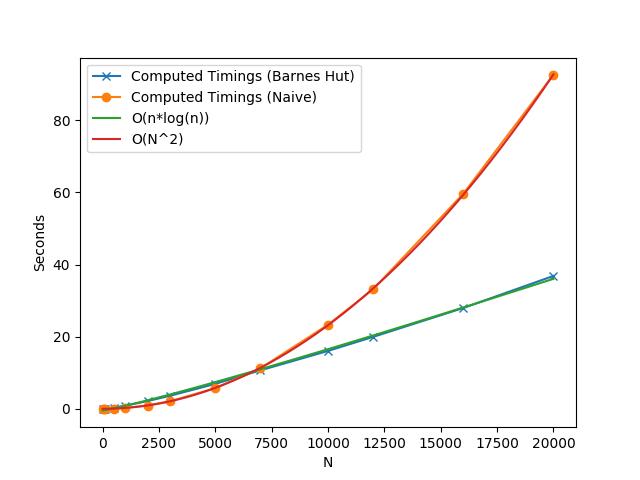
\includegraphics[width=8cm]{complexity_compare.png}
\caption{Time Complexity Plot}
\end{center}
\end{figure}
\newpage
\section{Appendix}
\begin{center}
    Quadtree Code
\end{center}
\begin{lstlisting}{language=C}
    void quadtree_add_particle(quadtree_t** tree, particle_t particle, box_bounds_t box) {

    if(*tree == NULL) {
        *tree = (quadtree_t*)malloc(sizeof(quadtree_t));
        (*tree)->mass = particle.mass;
        (*tree)->centre_of_mass = particle.position;
        (*tree)->box = box;
        (*tree)->north_west = NULL;
        (*tree)->north_east = NULL;
        (*tree)->south_west = NULL;
        (*tree)->south_east = NULL;
    } else if((*tree)->north_east == NULL && (*tree)->north_west == NULL && (*tree)->south_west == NULL && (*tree)->south_east == NULL) {
        
        particle_t particle_holder = {(*tree)->centre_of_mass, (*tree)->mass, {0.0, 0.0}, 1};
        
        double xcentre = ((*tree)->box.xlower + (*tree)->box.xupper)/2;
        double ycentre = ((*tree)->box.ylower + (*tree)->box.yupper)/2;

        if(particle_holder.position.x <= xcentre && particle_holder.position.y < ycentre) {
            box_bounds_t new_box = {box.xlower, xcentre, box.ylower, ycentre};
            quadtree_add_particle(&(*tree)->south_west, particle_holder, new_box);
        } else if(particle_holder.position.x > xcentre && particle_holder.position.y <= ycentre) {
            box_bounds_t new_box = {xcentre, box.xupper, box.ylower, ycentre};
            quadtree_add_particle(&(*tree)->south_east, particle_holder, new_box);
        } else if(particle_holder.position.x < xcentre && particle_holder.position.y >= ycentre) {
            box_bounds_t new_box = {box.xlower, xcentre, ycentre, box.yupper};
            quadtree_add_particle(&(*tree)->north_west, particle_holder, new_box);
        } else if(particle_holder.position.x >= xcentre && particle_holder.position.y > ycentre) {
            box_bounds_t new_box = {xcentre, box.xupper, ycentre, box.yupper};
            quadtree_add_particle(&(*tree)->north_east, particle_holder, new_box);
        }

        if(particle.position.x <= xcentre && particle.position.y < ycentre) {
            box_bounds_t new_box = {box.xlower, xcentre, box.ylower, ycentre};
            quadtree_add_particle(&(*tree)->south_west, particle, new_box);
        } else if(particle.position.x > xcentre && particle.position.y <= ycentre) {
            box_bounds_t new_box = {xcentre, box.xupper, box.ylower, ycentre};
            quadtree_add_particle(&(*tree)->south_east, particle, new_box);
        } else if(particle.position.x < xcentre && particle.position.y >= ycentre) {
            box_bounds_t new_box = {box.xlower, xcentre, ycentre, box.yupper};
            quadtree_add_particle(&(*tree)->north_west, particle, new_box);
        } else if(particle.position.x >= xcentre && particle.position.y > ycentre) {
            box_bounds_t new_box = {xcentre, box.xupper, ycentre, box.yupper};
            quadtree_add_particle(&(*tree)->north_east, particle, new_box);
        }

        (*tree)->centre_of_mass.x = ((*tree)->centre_of_mass.x*(*tree)->mass + particle.position.x*particle.mass)/((*tree)->mass + particle.mass);
        (*tree)->centre_of_mass.y = ((*tree)->centre_of_mass.y*(*tree)->mass + particle.position.y*particle.mass)/((*tree)->mass + particle.mass);
        (*tree)->mass += particle.mass;

    } else {
        (*tree)->centre_of_mass.x = ((*tree)->centre_of_mass.x*(*tree)->mass + particle.position.x*particle.mass)/((*tree)->mass + particle.mass);
        (*tree)->centre_of_mass.y = ((*tree)->centre_of_mass.y*(*tree)->mass + particle.position.y*particle.mass)/((*tree)->mass + particle.mass);
        (*tree)->mass += particle.mass;

        double xcentre = ((*tree)->box.xlower + (*tree)->box.xupper)/2;
        double ycentre = ((*tree)->box.ylower + (*tree)->box.yupper)/2;

        if(particle.position.x <= xcentre && particle.position.y < ycentre) {
            box_bounds_t new_box = {box.xlower, xcentre, box.ylower, ycentre};
            quadtree_add_particle(&(*tree)->south_west, particle, new_box);
        } else if(particle.position.x > xcentre && particle.position.y <= ycentre) {
            box_bounds_t new_box = {xcentre, box.xupper, box.ylower, ycentre};
            quadtree_add_particle(&(*tree)->south_east, particle, new_box);
        } else if(particle.position.x < xcentre && particle.position.y >= ycentre) {
            box_bounds_t new_box = {box.xlower, xcentre, ycentre, box.yupper};
            quadtree_add_particle(&(*tree)->north_west, particle, new_box);
        } else if(particle.position.x >= xcentre && particle.position.y > ycentre) {
            box_bounds_t new_box = {xcentre, box.xupper, ycentre, box.yupper};
            quadtree_add_particle(&(*tree)->north_east, particle, new_box);
        }
    }
} 
\end{lstlisting}

\begin{center}
    Forces code
\end{center}
\begin{lstlisting}{language=C}
    vector_t quad_force(quadtree_t* tree, particle_t particle, double theta_max) {
    vector_t f;
    vector_t r;
    double a;

    if(tree == NULL) {
        f.x = 0.0;
        f.y = 0.0;
    } else if(!vector_in_box(particle.position, tree->box) && (theta_bounds(tree, particle, theta_max) 
              || (tree->north_west == NULL && tree->north_east == NULL && tree->south_west == NULL && tree->south_east == NULL))) {
        r = r_vector(tree->centre_of_mass, particle.position);
        a = -(G * particle.mass * tree->mass) / norm3(r);
        f.x = a * r.x;
        f.y = a * r.y;
    } else {
        vector_t f1 = quad_force(tree->north_west, particle, theta_max);
        vector_t f2 = quad_force(tree->north_east, particle, theta_max);
        vector_t f3 = quad_force(tree->south_west, particle, theta_max);
        vector_t f4 = quad_force(tree->south_east, particle, theta_max);
        f.x = f1.x + f2.x + f3.x + f4.x;
        f.y = f1.y + f2.y + f3.y + f4.y;
    }
    return f;
}
}
\end{lstlisting}


\end{document}